\vspace*{-1mm}
The theoretical model for the transverse emittance growth caused by amplitude and phase noise in a CC was introduced in Chapter~\ref{Ch:CC_noise_theory}. In 2018, a dedicated experiment was conducted in the SPS to benchmark this model against experimental data and confirm the analytical predictions. In this chapter, the machine setup, the beam configuration and the instrumentation used for the emittance growth studies with $\CC$s in the SPS are presented.


\begin{sloppypar} % to fix \hbox too wide
The chapter is structured as follows: Section~\ref{sec:SPS_setup}
describes the experimental machine configuration. Thereafter, Section~\ref{sec:CC_SPS_setup} elaborates on the installation and the operational aspects of the CCs in the SPS. In Sections~\ref{sec:HT_info}-~\ref{sec:ABWLM_WallCurrentMonitor} the instruments used for the parameters of interest (see Chapter~\ref{Ch:CC_noise_theory}, Eq.~\eqref{eq:dey_an} and Eq.~\eqref{eq:dey_pn})  i.e. $\CC$ voltage, emittance and bunch length are discussed, including the post processing methods where it was performed by the author. The results of the experiment are presented in Chapter~\ref{Ch:2018_analyisis}.
\end{sloppypar}


\section{Machine and beam configuration}\label{sec:SPS_setup}
For studying the long-term emittance evolution a special mode of operation was set up in the SPS which is called "coast" (in other machines, it is referred to as storage ring mode) with bunched beams. In this mode, the bunches circulate in the machine at constant energy for long periods, from a few minutes up to several hours, similar to the HL-LHC case.

To make sure that the SPS can be used as a testbed for the emittance growth studies with $\CC$s an extensive preparatory campaign was carried out through 2012-2017~\cite{Calaga:1451286, Alekou_CC_coast_prep_2016, Antoniou:2649815}. The primary concern was the emittance growth that was observed in the machine from other sources than injected noise and will be referred to as the natural emittance growth in this thesis. The natural emittance growth needs to be well characterized and be kept sufficiently small in order to distinguish and understand the contribution from the $\CC$ noise. From these studies, it was concluded that the optimal coast setup is at high energies, with low chromaticity and bunches of low intensity as it minimises the natural emittance growth~\cite{Antoniou:2649815}. The highest energy for which the SPS could operate in "coast" was 270\,GeV and thus the experiments were performed at this energy. That limitation was introduced due to the rms power deposited in its magnets when operating at high energy for long period of time. Moreover, as the natural emittance growth was found to be a single bunch effect four bunches were used. That choice was made to reduce the statistical uncertainty of the measurements but not to increase the beam intensity.

During the experiment the Landau octupoles were switched off. Nevetherless, a residual non-linearity was present in the machine mainly due to multipole components in the dipole magnets~\cite{Carlà:2664976, Alekou:2640326}. Last, the transverse feedback system was switched off. The main machine and beam parameters used in the experiment of 2018 are listed in Table~\ref{tab:machine_beam_param_2018}. It should be noted, that no measurements of chromaticity are available from the day of the experiment. However it was ensured that the chromaticity was corrected to small positive values. 

\begin{table}[!hbt]
	\centering
   \caption{Main machine and beam parameters for the emittance growth studies with CCs in SPS in 2018.}
	\begin{tabu} to \textwidth {X[c,m] X[0.5c,m] X[0.5c,m] X[0.01c,m]}
		&&& \\[-6mm]
		\toprule \toprule
		\multicolumn{2}{l}{\textbf{Parameter}} &
		\multicolumn{2}{c}{\textbf{Value}} \\
		\bottomrule
      \multicolumn{2}{l}{Beam energy, $\symE$} & \multicolumn{2}{c}{270\,GeV} \\
      \multicolumn{2}{l}{Revolution frequency, $\frev$}  & \multicolumn{2}{c}{43.375\,kHz} \\
      \multicolumn{2}{l}{Number of proton per bunch, $\Nb$} & \multicolumn{2}{c}{3 $\times 10^{10}$ p/b} \\
      \multicolumn{2}{l}{Number of bunches}  & \multicolumn{2}{c}{4} \\
      \multicolumn{2}{l}{Bunch spacing}  & \multicolumn{2}{c}{524\,ns} \\
      \multicolumn{2}{l}{Main RF frequency, $\fRF$}  & \multicolumn{2}{c}{200.39\,MHz} \\ %200.3945
      \multicolumn{2}{l}{Main RF voltage, $\VRF$}  & \multicolumn{2}{c}{3.8\,MV} \\
      \multicolumn{2}{l}{Horizontal / Vertical betatron tune, $\Qx$ / $\Qy$}  & \multicolumn{2}{c}{26.13 / 26.18} \\
      \multicolumn{2}{l}{Horizontal / Vertical first order chromaticity, $\Qpx$ / $\Qpy$}  & \multicolumn{2}{c}{ $\sim$ 1.0 / $\sim$ 1.0} \\
      \multicolumn{2}{l}{Synchrotron tune, $\Qs$}  & \multicolumn{2}{c}{0.0051} \\
      \bottomrule
	\end{tabu}
   \label{tab:machine_beam_param_2018}
\end{table}

\section{Crab Cavities in the SPS}\label{sec:CC_SPS_setup}

For the SPS tests two prototype $\CC$s of the Double Quarter Wave (DQW) type, $\CC$1 and $\CC2$, were fabricated by CERN and were assembled in the same cryomodule, shown in Fig.~\ref{fig:DQW_cryomodule}~\cite{Zanoni:2017}. For its istallation For its installation an available space was found at the SPS Long Straight Section 6 (SPS-LSS6) zone. As this section is also used for the extraction of the beam to the LHC, the cryomodule was placed on a mobile transfer table~\cite{Calaga:2649807} which  moved the cryomodule in the beamline for the $\CC$ tests and out of it for the usual SPS operation without breaking the vaccum. For the noise induced emittance growth studies only $\CC$2 was used. Nevertheless, the parameters for both $\CC$s are shown in Table~\ref{tab:SPS_CC_main} for completeness. In case someone wants to repeat the study, the location of the $\CC$s along the SPS ring is also indicated.

\begin{figure}[h]
   \centering         
   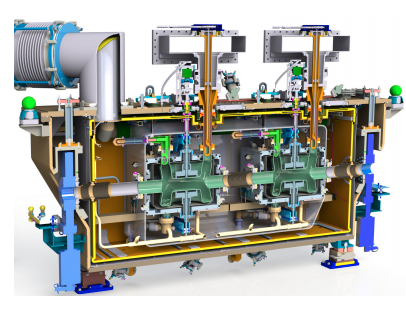
\includegraphics[width=0.8\textwidth]{images/Ch4/CC_cryomodule.png}
       \caption{Cross section view of the CC cryomodule~\cite{Zanoni:2017}. It has a total length of 3\,m~\cite{Baudrenghien:1520896} and at its core there are the two DQW cavities, which are illustrated with light green color.}
       \label{fig:DQW_cryomodule}
\end{figure}
% Couldn't find information on height, weight etc. Any idead where to look for spces?

% Photos from the cryomodule installation day: 1. https://home.cern/news/news/engineering/crabs-settled-tunnel (maybe good to show the scale?)
% 2. https://science.osti.gov/-/media/np/pdf/research/NP-Accel-RD-PI-Meeting/2019/Wu_2019FOA_PImeeting_crabcavity_Rev9.pdf?la=en&hash=B29283EDB3C704EC3EFD9DA23CA8DEA22076C88B


\begin{table}[!hbt]
   \begin{minipage}{\textwidth}
   %\centering
   \begin{centering}
   \caption{Crab cavities parameters for the emittance growth studies in SPS in 2018.}
   \begin{tabu} to \textwidth {X[c,0.1m] X[c,m] X[0.5c,m] X[0.5c,m]}
		&&& \\[-6mm]
		\toprule \toprule
		\multicolumn{2}{l}{\textbf{Parameter}} &
		\multicolumn{2}{c}{\textbf{Value}} \\
		\bottomrule
      \multicolumn{2}{l}{} & 	\multicolumn{1}{c}{\textbf{CC1}} & \multicolumn{1}{c}{\textbf{CC2}} \\
      \midrule
      \multicolumn{2}{l}{crabbing plane}  & \multicolumn{1}{c}{vertical} & \multicolumn{1}{c}{vertical} \\
      
      \multicolumn{2}{l}{s-location$^{\ast}$}  & \multicolumn{1}{c}{6312.72\,m} & \multicolumn{1}{c}{6313.32\,m} \\

      \multicolumn{2}{l}{$\CC$ voltage, $\VCC$}  & \multicolumn{1}{c}{0\,MV} & \multicolumn{1}{c}{$\sim$ 1\,MV} \\

      \multicolumn{2}{l}{$\CC$ frequency, $\fCC$}  & \multicolumn{1}{c}{400.78\,MHz} & \multicolumn{1}{c}{400.78\,MHz} \\ %400.789

      \multicolumn{2}{l}{Horizontal / Vertical beta function, $\beta_{x, CC}$ / $\beta_{y, CC}$}  & \multicolumn{1}{c}{29.24\,m / 76.07\,m} & \multicolumn{1}{c}{30.31\,m / 73.82\,m} \\

      \multicolumn{2}{l}{Horizontal / Vertical alpha function, $\alpha_{x, CC}$ / $\alpha_{y, CC}$} & \multicolumn{1}{c}{-0.88\,m / 1.9\,m} & \multicolumn{1}{c}{-0.91\,m / 1.86\,m} \\

      \multicolumn{2}{l}{Horizontal / Vertical dispersion, $D_{x, CC}$ / $D_{y, CC}$} & \multicolumn{1}{c}{-0.48\,m / 0\,m}  & \multicolumn{1}{c}{-0.5\,m / 0\,m} \\
      \arrayrulecolor{black}\bottomrule
	\end{tabu}
   \label{tab:SPS_CC_main}
   \end{centering} \footnotesize{$^\ast$ The s-location is reffered to the location of the elements along the SPS ring with respect to the start of the lattice i.e. element QF.10010 which is a focusing quadrupole.}
   \end{minipage}
\end{table}
% QF.10010  is the start of the SPS lattice --> https://layout.cern.ch/reports/mad?fileType=STANDARD&machineId=2180065&versionId=34464591 (access with sshuttle)
% The actual start of the lattice at 0 m is: %BEGI.10010. which is a marker (not a real element).

% Optics parameters for CC and diagnostics in 2018: https://cernbox.cern.ch/index.php/apps/files/?dir=/__myshares/SPS_MDs_2018%20(id%3A271128)/SPSMeasurementTools&#editor

\subsection{Operational considerations}

For the beam tests with the $\CC$ in the SPS the approach regarding the energy ramp and the adjustment of the phasing with the main RF system needed to be evaluated and they are briefly discussed here.

\normalsize{\textbf{Energy ramp}}\\
SPS recieves the proton beam at 26\,GeV from the PS. It was found that the ramp to higher energies could not be performed with the $\CC$ on, as the beam was getting lost while crossing one of the vertical betatron sidebands due to resonant excitation~\cite{Rama_Paris_persentation}. Therefore, it was established that the acceleration has to be performed with the $\CC$ off and its voltage must be set up only after the energy of interest has been achieved. It is worth noting that this approach will also be used in the HL-LHC.

\normalsize{\textbf{Crab Cavity - main RF synchronisation}}\\
It was important to ensure that during the "coast" the beam will epxeriene the same kick from the $\CC$ each turn. In other words the SPS main RF system operating at 200\,MHz needed to be synchronous with the $\CC$ operating at 400\,MHz. Due to the larger bandwidth of the SPS main RF system the $\CC$ was used as a master. Therefore the $\CC$ was operating at a fixed frequency and phase, while the main accelerating cavities were adjusted to the exact half of the $\CC$ frequency (see values at Tables~\ref{tab:machine_beam_param_2018} and~\ref{tab:SPS_CC_main}) and were re-phased so that they become synchronous with the crabbing signal. For the studies at 270\,GeV the synchronisation took place at the end of the ramp to the coast energy and shortly after the cavity was switched on~\cite{BE_seminar}.

% Steps for synchronisation: 1) SPS main RF was set at the exact half of the main RF. 2) The phase was adjusted. 3) The frequency needed to be re-adjusted slightly again such is it becomes the exact half of it.
% Nice explanation of the synchronisatio: https://journals.aps.org/prab/pdf/10.1103/PhysRevAccelBeams.24.062001
% For studies at the injection energy of 26\,GeV this synchronisation took place shortly after the injection. 


% Plotting figures in this section: /eos/user/n/natriant/2021/CC_MD_2021_summary/2018_HT_monitor
\section{SPS Head-Tail monitor}\label{sec:HT_info}
% info on the bandwidth of HT monitor https://indico.cern.ch/event/1044711/contributions/4389270/attachments/2264278/3844129/CCNoise_SPS_MDs.pdf

The SPS is equipped with a high bandwidth pick-up of approximately 2\, GHz allowing to resolve the intra-bunch motion. This instrument is called Head-Tail (HT) monitor and was originally designed for measuring chromaticity and transverse isntabilities. However, in the SPS $\CC$ tests, the HT monitor was the main diagnostic device deployed for the measurement of the crabbing and the calibration of the $\CC$ voltage. Therefore its use as a crabbing diagnostic should be explained here. The methods and procedures described in this section were developed at CERN and they are described here for the completness of the thesis.

 In the first part of this section some general information on the instrument along with example signals will be presented. Subsequently, the post processing of the HT signal in the presence of the $\CC$ will be discussed. Last, the calibration of the $\CC$ voltage from the HT data is described. The experimental data presented in this section were acquired at the SPS injection energy of 26\,GeV with only one $\CC$, $\CC$1, at phase $\phiCC=0$ for simplicity. That energy of 26\,GeV was chosen to provide a better understanding of the methods used as the orbit shift from the $\CC$ kick is stronger and thus more visible than in higher energies.


\normalsize{\textbf{General information}}\\
As already mentioned, the HT monitor is a high bandwidth version of a standard beam position monitor, which means that it can measure the transverse displacement within the bunch. This makes it ideal for the measurement of the intra-bunch offset caused from the $\CC$ kick. Its reading consists of the sum ($\Sigma$) and the  difference ($\Delta$) of the electrode signals of a straight stripline coupler (Fig.~\ref{fig:SPS_HT_diagram})~\cite{Jones:987561, Levens:2313358} over a defined acquisition period. The sum signal is the longitudinal line density while the difference signal corresponds to the intra-bunch offset. The system operates at time scale where the signals are given as a function of the position within the bunch.

\begin{figure}[h]% Edit figure in: Goodle Docs/Doctoral/2022/Thesis/Ch4
   \centering         
   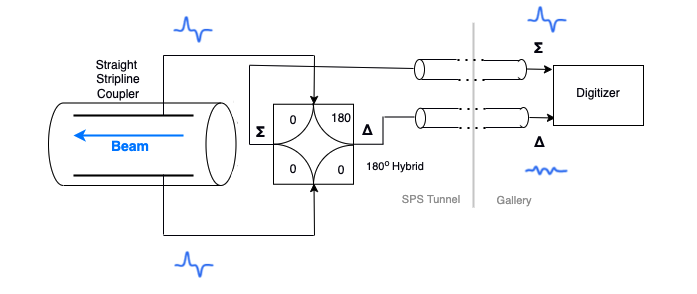
\includegraphics[width=1.0\textwidth]{images/Ch4/HT_monitor_sketch.png}
       \caption{Diagram of the SPS HT monitor~\cite{Levens:2313358}. The beam is passing through a straight stripline coupler which is followed by a 180$^\circ$hybrid. This configuration provides the sum ($\Sigma$) and the difference ($\Delta$) signal of the two electrodes.} %, which correspond to the longitudinal line density and intra-bunch offset, respectively.} 
       \label{fig:SPS_HT_diagram}
\end{figure}
% what is a 180 hybrid. A 180° Hybrid Coupler is a four port device that is used either to equally split an input signal with a 180° phase shift between the ports or to combine two signals that are 180° apart in phase. (from google)

The raw signals from the HT monitor require a specific post-processing procedure, which is described in Ref.~\cite{Levens:2313358}, in order to give useful information. Figure~\ref{fig:HT_example_signals} shows some example signals obtained from the HT monitor after the basic post-processing is applied. Moreover, Fig.~\ref{fig:HT_example_signals_2D} shows a 2D representation of the HT monitor reading. It is worth noting here that in the specific example a clear modulating pattern in time of the vertical intra-bunch offset (vertical $\Delta$) signal is observed. This is a result of the phase slip between the $\CC$ and the main RF system because they are not yet synchronised. 
% COMMENT: The Ref.~\cite{Levens:2313358} refers to the LHC HT monitor but the same applies for SPS as it is the same device.

\begin{figure}[!h]
   \centering         
   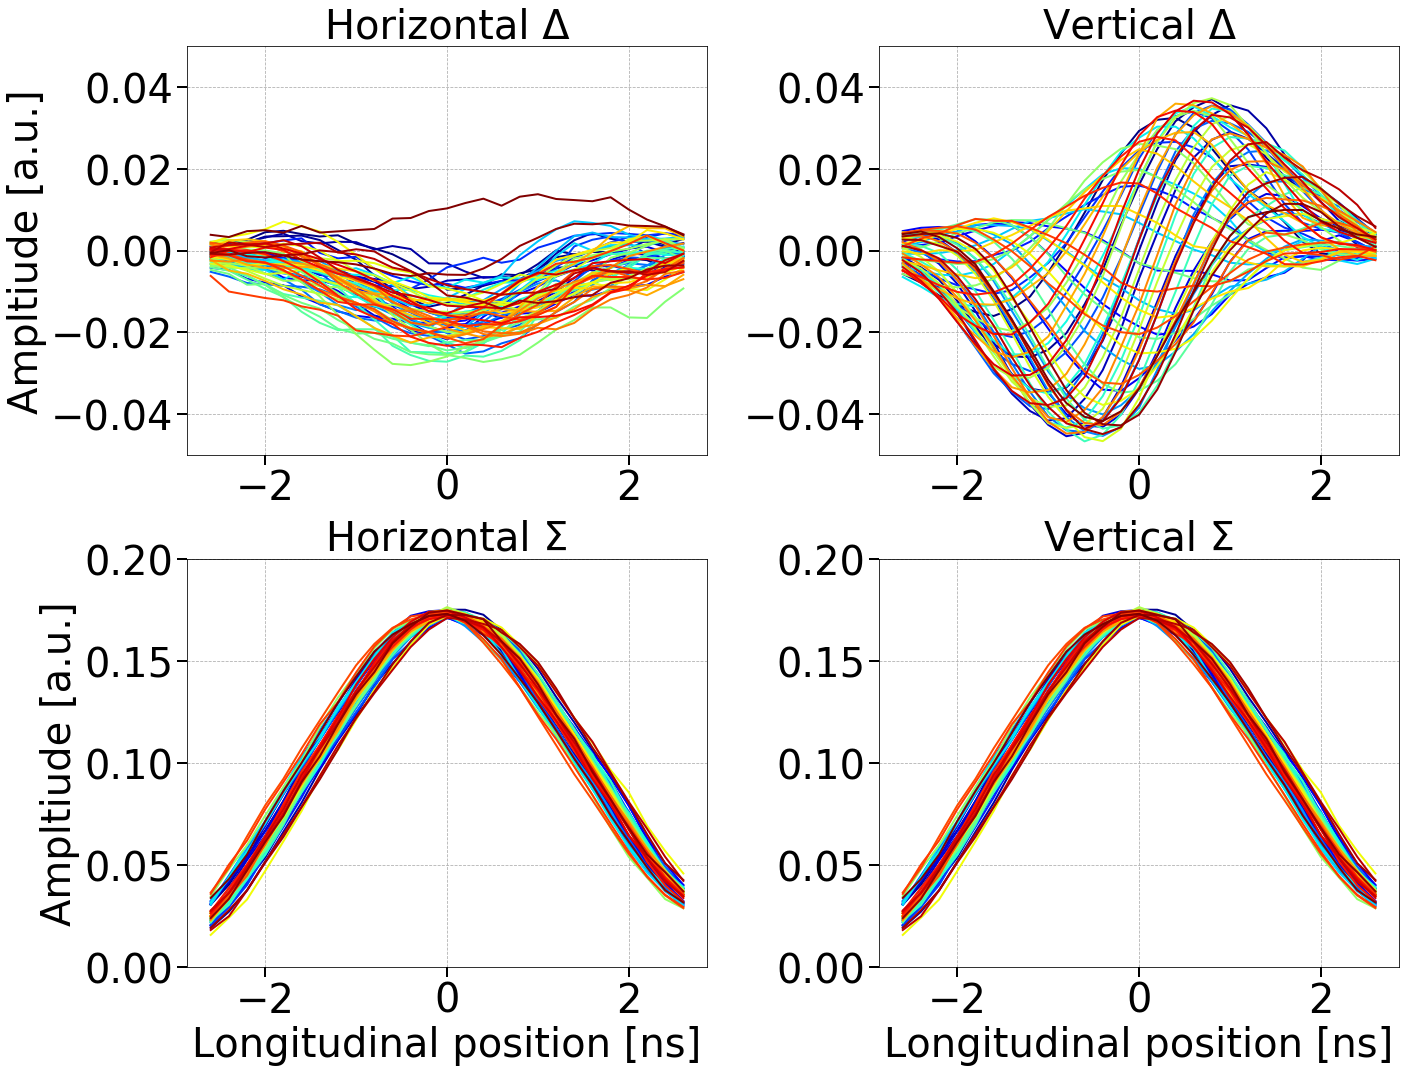
\includegraphics[width=0.8\textwidth]{images/Ch4/HT_1D__20180530_135105exampleAcq_4thesis_turnsStart0_Stop6000_step100_new.png}
       \caption{Example difference and sum signals (top and bottom plots, respectively) from the HT monitor, in time scale, with respect to the longitudinal position within the bunch over several SPS revolutions, after the basic post processing (Ref.~\cite{Levens:2313358}) but before the baseline correction. The different colors indicate the signals from different turns (every 100 turns). } % mention every how many turns you plot, shows an indication of how fast is the instrument.
       \label{fig:HT_example_signals}
\end{figure}

\begin{figure}[!h]
   \centering         
   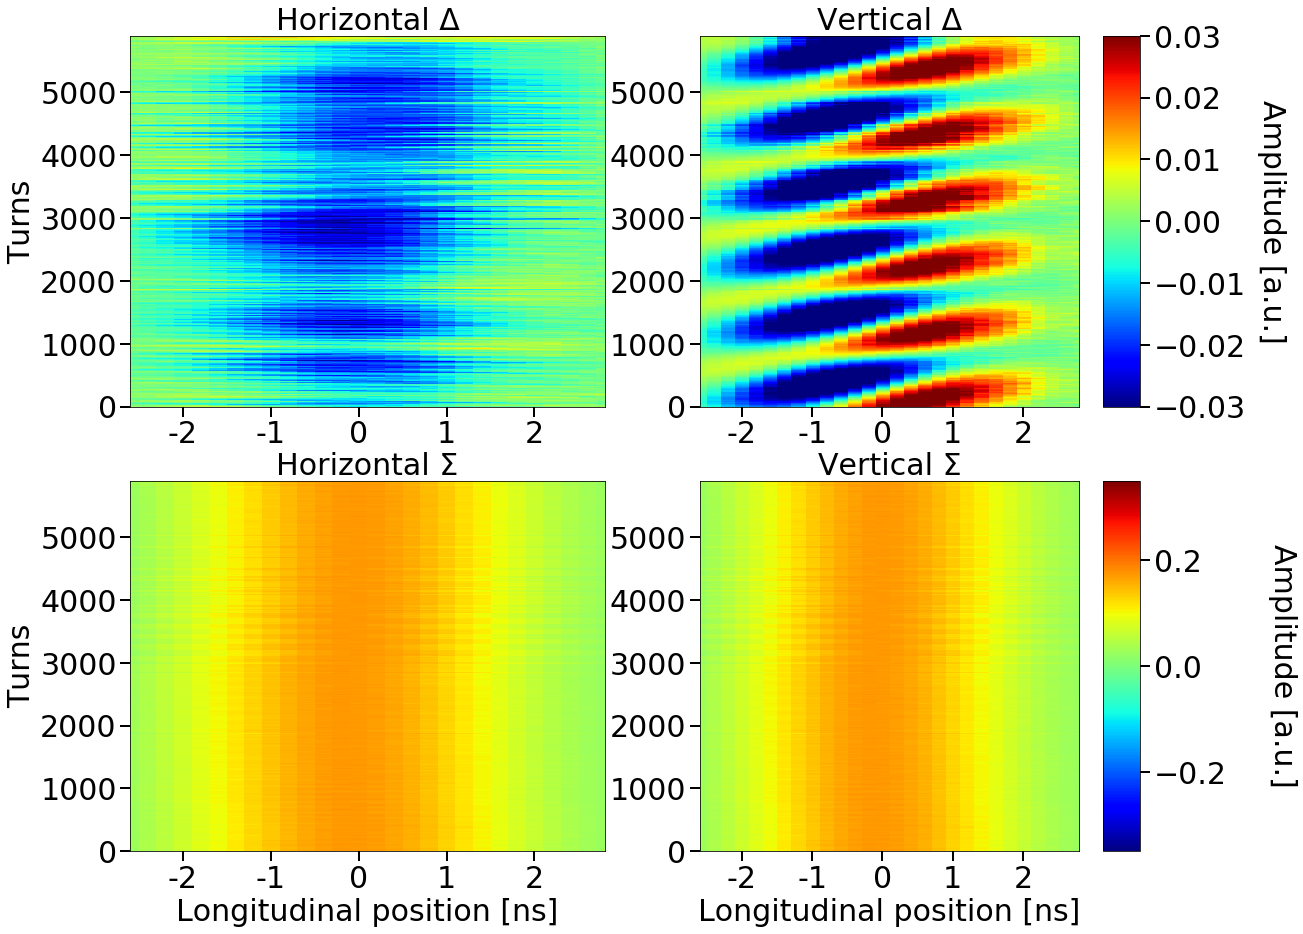
\includegraphics[width=0.9\textwidth]{images/Ch4/HT_2D__20180530_135105_colorbar_new_version.png}
       \caption{2D representation of example difference and sum signals with respect to the longitudinal position within the bunch obtained from the HT monitor over several SPS revolutions.}
       \label{fig:HT_example_signals_2D}
\end{figure}


\subsection{Post processing in the presence of Crab Cavities}\label{subsec:HT_post_process_CC}
To obtain useful information from the HT monitor signal in the presence of the $\CC$s there are a few steps that differ from the standard post processing procedure and they are desribed below.

\normalsize{\textbf{Head-Tail monitor baseline correction}}\\
The HT monitor measurement has a baseline on the difference signal which needs to be removed. The baseline is a result of orbit offsets and non-linearities of the instrument and is constant from turn to turn~\cite{Levens:2313358}. Therefore, during the normal post processing procedure (without $\CC$s), the baseline is computed as the mean of the difference signals over all turns and then the correction is achieved by subtracting this static offset from the signal of each turn. However, in the SPS tests, where the $\CC$s are well synchronised with the main RF system (Section~\ref{sec:CC_SPS_setup}), the crabbing signal is also a static intra-bunch position offset and thus would also be removed with the usual method. Because of technical limitations it was not feasible to switch off the $\CC$ for those kind of measurements. Thus, the following technique was used. 
% CC effect average out over time

For the $\CC$ experiments a reference measurement had first to be made with the $\CC$ not being synchronous with the main RF system. The baseline was computed as the mean of the difference signals over this reference period and subsequently it was subtracted from the average of the difference signals acquired after the synchronisation (Fig~\ref{fig:HT_baseline_correction}). The datasets before and after synchronisation are easily distinguishable in the 2D HT monitor reading as displayed in Fig.~\ref{fig:HT_baseline_correction_measurements_2D}


\begin{figure}[!h]
   \centering         
   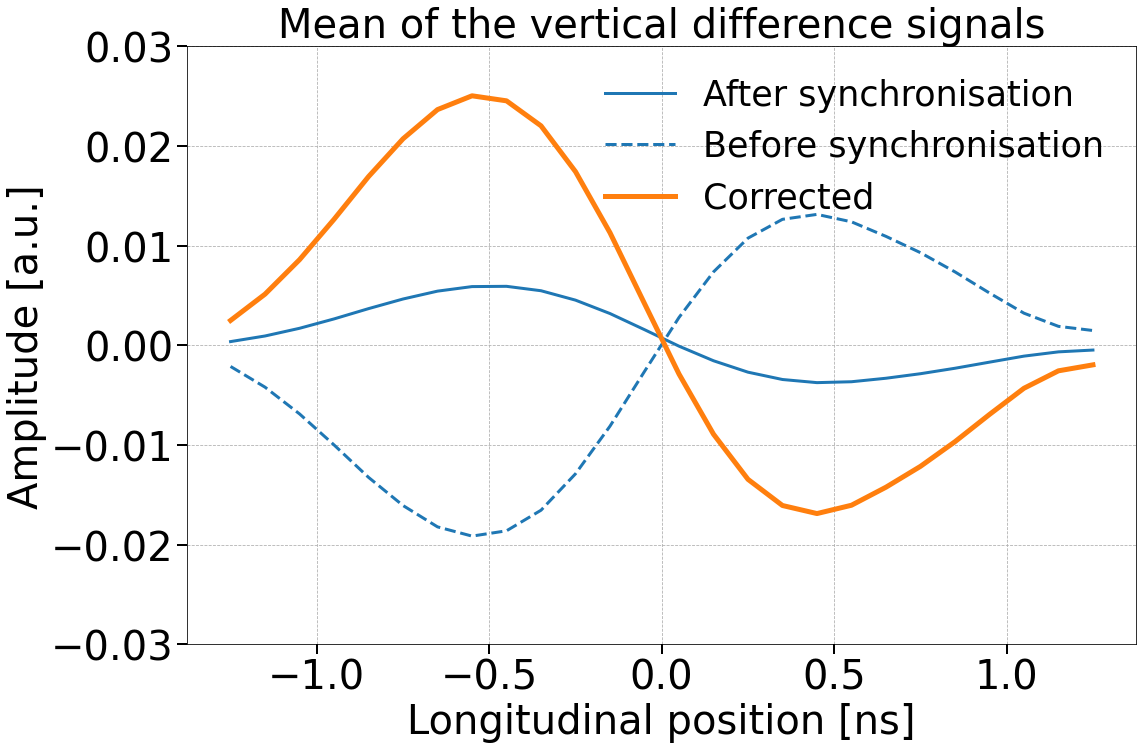
\includegraphics[width=0.65\textwidth]{images/Ch4/HT_measures_vs_reference_vs_corrected__20180530_135105_baseline_correction_new_version.png}
       \caption{HT monitor baseline correction for the SPS CC tests. The baseline signal (blue dashed line) refers to the mean of the difference signals acquired before the CC - main RF synchronisation. The measured signal (blue solid line) corresponds to the mean of the difference signal acquired after the synchronisation. Last, the corrected signal (orange solid line) is obtained after subtracting the baselin from the measured signal.}
       \label{fig:HT_baseline_correction}
\end{figure}

\begin{figure}[!h]
   \centering         
   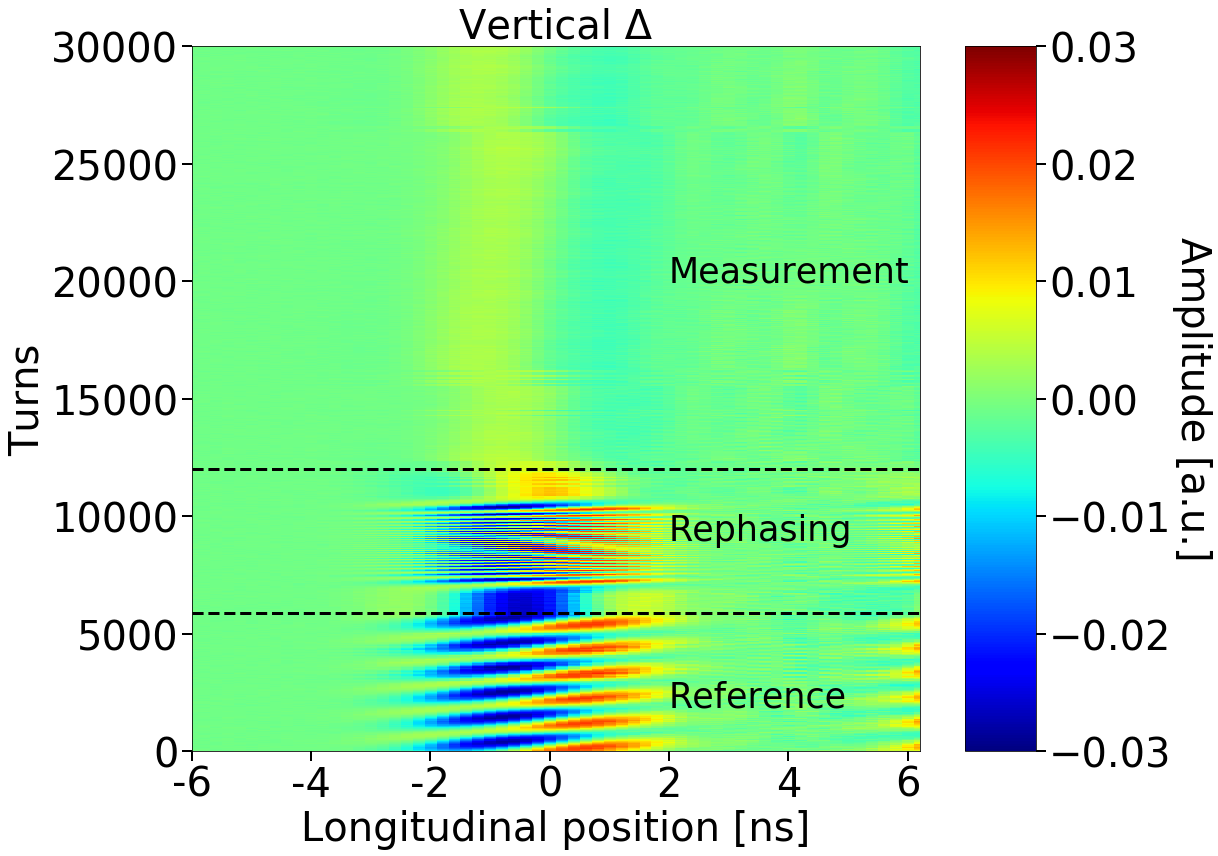
\includegraphics[width=0.7\textwidth]{images/Ch4/HT_2D__20180530_135105_before_after_sunchronisation_new_version.png}
       \caption{HT acquistions before and after the synchronisation of the SPS main RF with the CC.}
       \label{fig:HT_baseline_correction_measurements_2D}
\end{figure}

\normalsize{\textbf{Head-Tail monitor callibration}}\\
The last step to make the HT acquisitions meaningful is to convert the measured intra bunch offset, mean of the difference signals after the $\CC$ - main RF synchronisation and after the baseline correction, from arbitrary units to millimeters. The scaling is achieved by division with the mean of the sum signals after the synchronisation and with a normalisation factor which is provided by the calibration of the HT monitor~\cite{PhysRevAccelBeams.22.112803}. The normalisation factor for the SPS was measured at 0.1052 in 2018~\cite{HT_calibration_2018}. Figure~\ref{fig:HT_baseline_correction_crabbing_mm} shows the intra-bunch offset from the $\CC$ kick in millimeters and after the baseline correction. 


\begin{figure}[!h]
   \centering         
   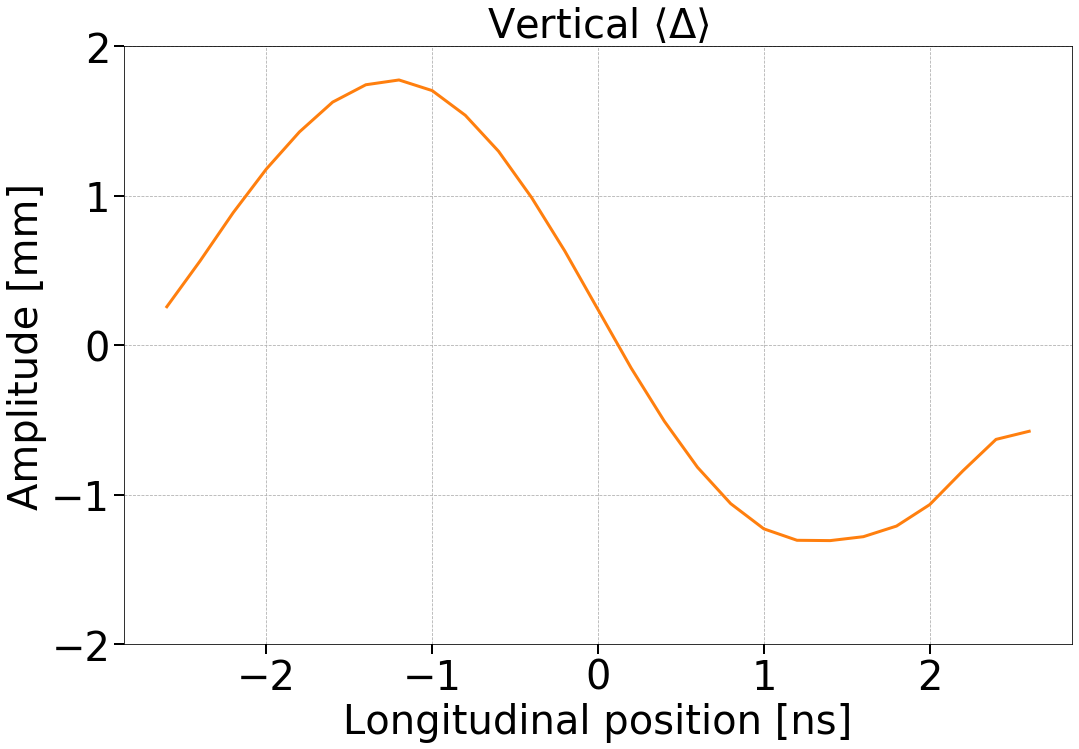
\includegraphics[width=0.65\textwidth]{images/Ch4/HT_corrected__20180530_135105_baseline_correction_new_version.png}
       \caption{Intra-bunch offset from the CC kick expressed in millimeters after the removal of the baseline.}
       \label{fig:HT_baseline_correction_crabbing_mm}
\end{figure}


 \subsection{Crab Cavity voltage calibration}\label{sec:Vcc_calibration}
 This section discusses the beam based measurement of the $\CC$ voltage from the HT monitor signal. The calibration was performed by using Eq.~\eqref{eq:CC_orbit_shift_Chao} to calculate the kick required to reconstruct the measured intra-bunch offset. Equation~\eqref{eq:CC_orbit_shift_Chao}, which is obtained from Eq.\,(1) from chapter 4.7.1 in Ref.~\cite{Chao:1490001}, gives the vertical orbit shift (in meters) from the $\CC$ kick, $\theta$, at the HT monitor location as follows:


\begin{equation}\label{eq:CC_orbit_shift_Chao}
   \Delta y_{,HT} = \frac{\sqrt{\beta_{y, HT}}}{2 \sin(\pi \Qy)} \theta \sqrt{\beta_{y, CC}} \cos(\pi \Qy - \mid \psi_{y, HT} - \psi_{y, CC} \mid),
\end{equation}

where $\beta_y$ is the beta function, $\Qy$ is the tune, and $\mid \psi_{y, HT} - \psi_{y, CC} \mid$ between the $\CC$ and the HT monitor in tune units. The same applies for the horizontal plane. The subscripts HT and CC indicate quanities at the location of the HT monitor and CC respectively.

The deflection from the $\CC$ is written as $\theta = - \frac{q V(t)}{\symE}$, where $q$ is the charge of the particle, $\symE$ the beam energy and $V_{CC}(t) = \VCC \sin(2 \pi \fCC t + \phiCC) $ is the voltage that a particle experiences while passing through the $\CC$. In the context where the HT monitor measures the signal as a function of time, $t$, the voltage in the above formula is expressed accordingly as $V_{CC}(t)$, where $t=0$ the center of the bunch.

% 1. locally PhD_projects/CC_MD_2021_summary/HT_monitor/2018_HT_monitor
% 2. lxplus: cernbox/2021/CC_MD_2021_summary/HT_monitor/2018_HT_monitor
\begin{figure}[!h]
\centering         
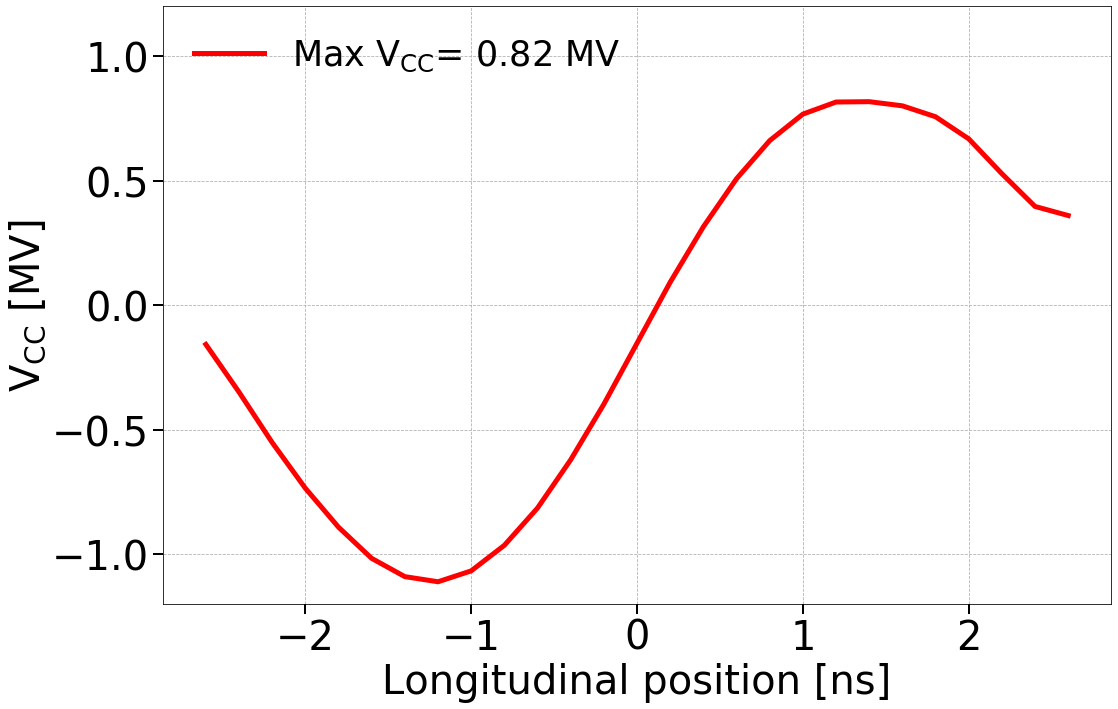
\includegraphics[width=0.65\textwidth]{images/Ch4/HT_VCC_callibration_20180530_135105.png}
    \caption{CC voltage calibration from the HT monitor. The measured CC voltage, considered as half the peak to peak amplitude of the signal, is 0.96\,MV.}
    \label{fig:VCC_from_HT_monitor_measurement}
\end{figure}

It should be noted here, that the measured intra-bunch offset, $\Delta y_{, HT}$, is inserted in Eq.~\eqref{eq:CC_orbit_shift_Chao} after removing the baseline and converting it to millimeters as discussed in Section~\ref{subsec:HT_post_process_CC}. Figure~\ref{fig:VCC_from_HT_monitor_measurement} illustrates the cavity voltage computed from the HT signals shown already in this section. The corresponding beam and optic parameters are listed in Table~\ref{tab:SPS_HT_CC}.

\begin{table}[!hbt]
	\begin{minipage}{\textwidth}
   \begin{centering}
   \caption{Parameters for computing the CC voltage from the example HT monitor measurements discussed in this chapter.}
	\begin{tabu} to \textwidth {X[c,m] X[0.01c,m] X[0.01c,m] X[0.01c,m]}
		&&& \\[-6mm]
		\toprule \toprule
		\multicolumn{2}{l}{\textbf{Parameter}} &
		\multicolumn{2}{c}{\textbf{Value}} \\
		\bottomrule
      \multicolumn{2}{l}{Beta function at the HT monitor, $\beta_{y, HT}$}& \multicolumn{2}{c}{49.19\,m} \\
      \multicolumn{2}{l}{Phase advance between the start$^{\ast}$ of the lattice and the HT monitor, $\psi_{y, HT}$} & \multicolumn{2}{c}{15.68 $\times$ 2$\mathrm{\pi}$} \\
      \multicolumn{2}{l}{Beta function at the $\CC$1, $\beta_{y, CC1}$}& \multicolumn{2}{c}{76.07\,m} \\
      \multicolumn{2}{l}{Phase advance between the start$^{\ast}$ of the lattice and $\CC$1, $\psi_{y, CC1}$} & \multicolumn{2}{c}{23.9 $\times$ 2$\mathrm{\pi}$} \\
      \multicolumn{2}{l}{Vertical betatron tune, $\Qy$} & \multicolumn{2}{c}{26.13} \\
      \multicolumn{2}{l}{Beam energy, $\symE$} & \multicolumn{2}{c}{26\,GeV} \\
      \bottomrule
	\end{tabu}
   \label{tab:SPS_HT_CC}
   \end{centering} \footnotesize{$^\ast$ The start of the lattice is considered the element QF.10010 which is a focusing quadrupole.}
   \end{minipage}
\end{table}

\normalsize{\textbf{Estimation of the amplitude and the uncertainty of the measurement}}\\
It is clear from Fig.~\ref{fig:VCC_from_HT_monitor_measurement} that the reconstructed $\CC$ voltage, $\VCC(t)$, is not centered around zero. This voltage offset is not a systematic error as it is not in the same direction and has different value for each measurement. In this case, the amplitude of the signal is defined as half the peak to peak amplitude, $\VCC = V_{CC, p-p}/2$. Note that the peak to peak amplitude, $V_{CC, p-p}$, is the difference between the maximum positive and negative peaks of the signal. The uncertainty in the amplitude is defined as the offset that needs to be added or subtracted to the signal such as it is centered around zero. In other words the uncertainty, $\Delta \VCC$, is defined half the sum of the maximum positive and negative peaks of the signal. Figure ... shows the peak to peak amplitude, $V_{CC, p-p}$, the signal amplitude, $\VCC$, and its uncertainty, $\Delta \VCC$, for the reconstructed $\CC$ voltage, $\VCC(t)$.



\normalsize{\textbf{Reconstruction of crabbing}}\\
Additionally, the measurements from the HT monitor were used for reconstructing the crabbing and representating schematically the beam projection {\color{red}in the transverse plane}. The technique for reconstructing the crabbing was developed at CERN in 2018 and was extensively used throught the experimental campaign with $\CC$s since (together with the calibrated voltage) it gives a straightforward estimate of the applied $\CC$ kick, as illustrated in Fig.~\ref{fig:crabbing_reconstruction_HT_monitor}. \\ 

%The reconstruction of the crabbing from the HT monitor measurements and the physical illustration of it are presented here. 
%This made it a very useful tool during the experiments as it provided a direct validation of the effect of the $\CC$ kick on the beam. 

To obtain this schematic representation, which is practically a density plot, of the effect of the CC kick on the beam one needs to multiply the measured longitudinal profile, mean of the sum signals acquired after the synchronisation, with the measured intra-bunch offset, mean of the differene signals acquired after the synchronisation. An example of this is shown in Fig.~\ref{fig:HT_baseline_correction_crabbing_mm}. For the transverse plane a gaussian distribution is considered with $\sigma$ obtained from the wire scanner (addressed in more detail in the following section). The color code of Fig.~\ref{fig:crabbing_reconstruction_HT_monitor} is normalised to the maximum intensity within the bunch.

\begin{figure}[!h]
   \centering         
   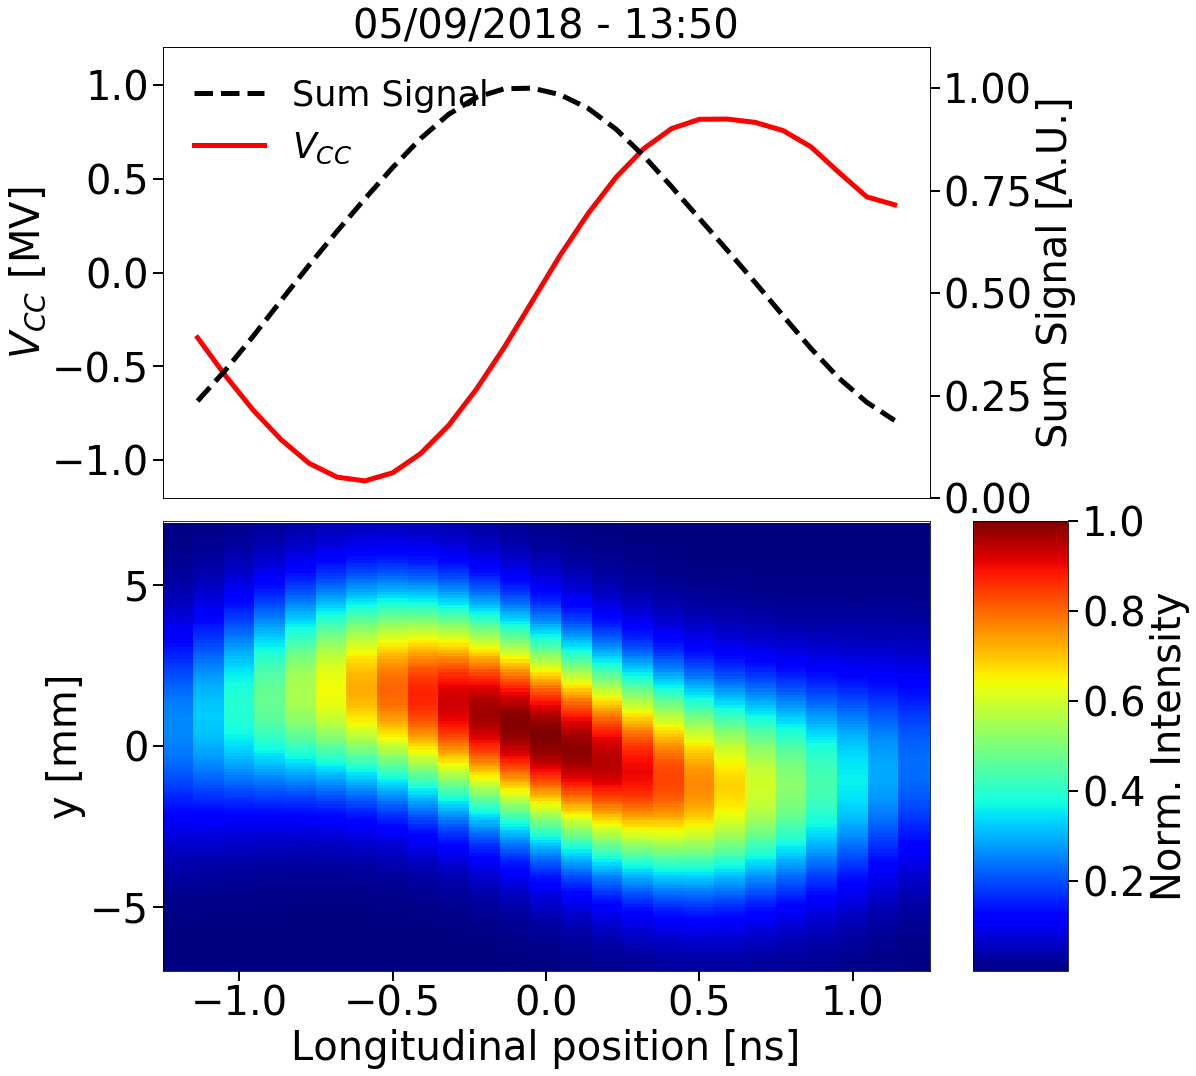
\includegraphics[width=0.7\textwidth]{images/Ch4/HT_crabVoltage__20180530_135105_crabbing_only.png}
       \caption{Illustration of the crabbing from the HT monitor signal. CC voltage and sum signal (longitudinal line density) measured from the HT monitor (top) together with the density plot (bottom) which visualises the effect of the CC kick in the beam.}
       \label{fig:crabbing_reconstruction_HT_monitor}
\end{figure}
   



\section{SPS Wire Scanners}

The SPS is equipped with Wire Scanners (WS) to measure the transverse beam emittance. The SPS WS system is described in detail in Ref.~\cite{BOSSER1985475, Berrig:1972478}. For the SPS tests, the emittance was measured with WS both for the horizontal and vertical plane (BWS.51995.H and BWS.41677.V respectively).

The working principle is shown in Fig.~\ref{fig:SPS_WS_ROT}. A thin wire rapidly moves across the proton beam and a shower of secondary particles is generated. The signal from the secondary particles is then detected by a system of scintillator and photomultiplier (PM) detectors outside of the beam pipe. By measuring the PM current as a function of wire position over multiple turns the transverse beam profile is reconstructed. An example of a vertical profile is shown in Fig.~\ref{fig:WS_example_V_profile}.

\begin{figure}[!h]
   \centering         
   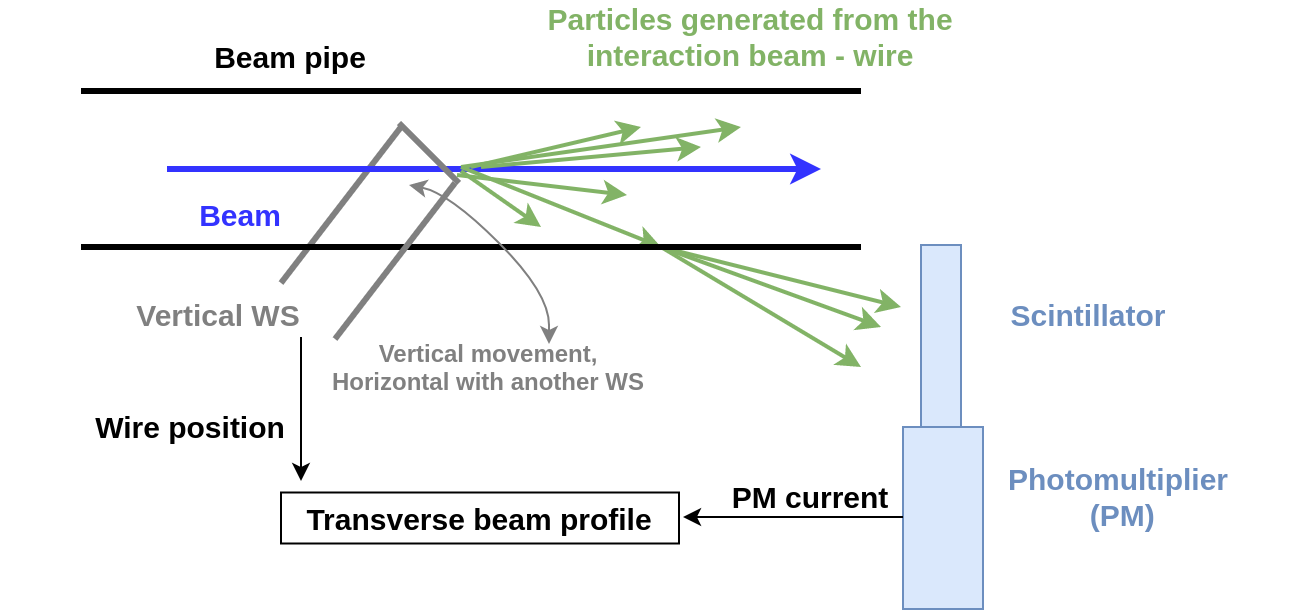
\includegraphics[width=0.8\textwidth]{images/Ch4/Wire_scanner.png}
       \caption{Sketch of the SPS rotational wire scanners~\cite{Berrig:1972478}. The wire moves across the proton beam generating secondary particles which are then detecting by a scintillator and a photomultiplier. From the measured photomultiplier current the beam profile is reconstructed.}
       \label{fig:SPS_WS_ROT}
\end{figure}


\normalsize{\textbf{Fitting of transverse profiles}}\\
To obtain the beam size, $\sigma$, the transverse profiles from each scan are fitted with a four-parameter gaussian function:

\begin{equation}\label{eq:4p_gauss}
   f(x) = k + A e^{-\frac{(x-\mu)^2}{2 \sigma^2}},
\end{equation}

where $k$ is the signal offset of the PM, $A$ is the signal amplitude, $\mu$ is the mean of the Gaussian distribution and $\sigma$ its standard deviation. The uncertainty of the measured beam size, $\Delta \sigma$, is defined as the one standard deviation error on $\sigma$ which is computed from the square root of the diagonal elements of the covariant matrix.
%https://docs.scipy.org/doc/scipy/reference/generated/scipy.optimize.curve_fit.html



% Location where the figure was produced: /eos/user/n/natriant/2020/WS_analysis
\begin{figure}[!h]
   \centering         
   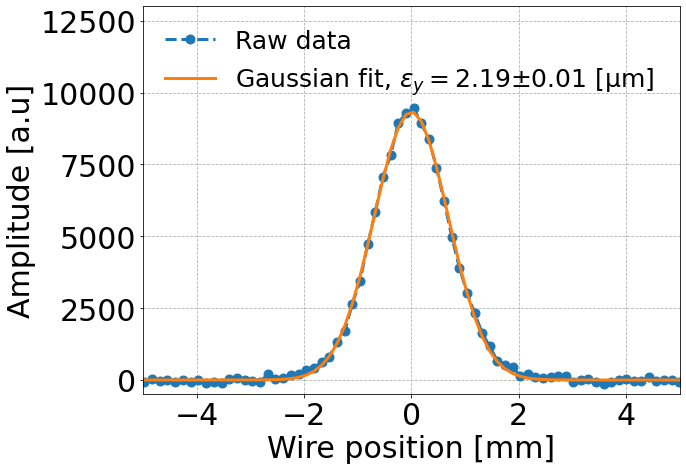
\includegraphics[width=0.6\textwidth]{images/Ch4/SPS.BWS.41677.V_ROT_2018-09-05 15_45_01.33500_raw_and_fit.png}
       \caption{Vertical beam profile obtained from the BWS.41677.V instrument. The measured data points (light blue) are fitted with a four parameter Gaussian (orange) to obtain the beam size. The calculated emittance is also shown.}
       \label{fig:WS_example_V_profile}
\end{figure}
   


The general formula for computing the normalised beam emittance from the beam size, $\sigma$ is given by:
\begin{equation}\label{eq:emittance_from_WS}
   \centering
   \epsilon = \frac{\sigma^2}{\beta_{WS}} \betarel \gammarel ,
\end{equation}

where $\sigma$ is the beam size, $\beta_{WS}$ the beta function at the WS location and $\betarel, \gammarel$ the relativistic parameters.


Note that, in the 2018 SPS operational configuration, the dispersion was small in the WSs location and thus its contribution to the beam size was considered to be negligible \footnote{The dispersion at BWS.51995.H location in 2018 was $D_x$= -15\,mm. At 270\,GeV, the energy spread, $\delta$, is of the order of $\mathrm{10^{-4}}$. Thus, from Eq.~\eqref{eq:emit_from_beam_size} the horizontal normalised emittance from the dispersion is foreseen at the order of $\mathrm{10^{-11}}$. Comparing to the observed beam size during the CC tests of a few microns the dispersion is negligible}. For the $\CC$ studies at 270\,GeV beam energy, the 
beta functions were 81.5\,m and 62.96\,m at the locations of the horizontal and vertical WS respectively, while $\betarel \gammarel$ equals 287.8.

Assuming that the relativistic parameters and the beta fucntion are free of error, the uncertainty of the computed emittance, $\Delta \epsilon$, at a dispersion free region, depends only on the uncertainty of the measured beam size, $\Delta \sigma$, as:

\begin{equation}\label{eq:emittance_from_WS_uncertainty}
   \centering
   \frac{\Delta \epsilon}{\epsilon} = \sqrt{\left(2\frac{\Delta \sigma}{\sigma} \right)^2} = 2\frac{\Delta \sigma}{\sigma}.
\end{equation}


\normalsize{\textbf{Further considerations}}\\
It is worth noting here that during each measurement with the WS the beam profile is actually acquired twice as the wire crosses the beam in the forward direction (IN scan) and then in the reverse direction (OUT scan). For the 2018 measurements the emittance values obtained from IN and OUT scans, $\epsilon_\mathrm{IN} \pm \Delta \epsilon_\mathrm{IN}$ and $\epsilon_\mathrm\mathrm{OUT} \pm \Delta \epsilon_{OUT}$ ,were found to be very similar. In the analysis of the 2018 measurements, the average emittance from the two scans, $\epsilon_\mathrm{avg} = \langle \epsilon_\mathrm{IN}, \epsilon_\mathrm{OUT}\rangle$ , is used. The uncertainty on the averaged emittance, $\Delta \epsilon_\mathrm{avg}$, is computed as:

\begin{equation}\label{eq:avg+emittance_from_WS_uncertainty}
   \Delta \epsilon_\mathrm{avg} = \sqrt{\Delta \epsilon_1 ^2 + \Delta \epsilon_2 ^2},
\end{equation}

where $\Delta \epsilon_1$ is the standard deviation (SD) of the $\epsilon_\mathrm{IN}$ and $\epsilon_\mathrm{OUT}$ and $\Delta \epsilon_2=\frac{1}{2}\sqrt{ \Delta \epsilon_\mathrm{IN}^2 + \Delta \epsilon_\mathrm{OUT}^2}$.


Finally, some emittance increase is expected during each wire scan, due to multiple Coulomb scattering. This effect has been extensively studied in Ref.~\cite{Roncarolo:1481835}. For the rotational SPS WS and the energy of 270\,GeV, at which the $\CC$ experiments were performed the expected emittance growth from the WS is expected to be small. However, a conservative number of scans were carried, $\sim$ 20 scans per bunch and per plane during $\sim$ 1 hour, in order to minimise the contribution from this effect.

\section{ABWLM and Wall Current monitor}\label{sec:ABWLM_WallCurrentMonitor}

\begin{sloppypar}
The bunch length was measured with two different instruments the ABWLM (A for RF, Beam, Wideband, Longitudinal, Measurement)~\cite{ABWLM} and the Wall Current monitor~\cite{Papotti:1124099}. The ABWLM measures the longitudinal profiles from which the bunch length is computed by performing a gaussian fit. The Wall Current monitor acquirest not just the longitudinal profiles but also the longitudinal beam position relative to the monitor i.e. the beam arrival with respect to the reference. The bunch length is estimated by computing the full width half maximum of the profiles and then using it to estimate the sigma of a gaussian distribution. No further details on the operation of these instruments are discussed here as the offline analysis was not performed by the author.
\end{sloppypar}


% beam position relative to monitor
